\documentclass[12pt]{article}

\usepackage[utf8]{inputenc}
\usepackage[colorlinks,linkcolor=red]{hyperref}
\usepackage{graphicx}

\title{
    {Paper Note}\\
    {\large "GhostNet: More Features from Cheap Operations"} \\
    {\small Paper Link: \href{https://arxiv.org/pdf/1911.11907.pdf}{CVPR 2020}}
}

\author{Lisen Dai}
\date{Nov 8, 2020}

\begin{document}
    \maketitle
    \section{
        Background
    }
        \subsection{
            Problem
        }
            Traditional CNNs usually need a large number of parameters and floating point operations (FLOPs) to achieve a satisfactory accuracy. \\
        \subsection{
            Previous Work
        }
            1. Network pruning. \\
            2. Low-bit quantization. \\
            3. Knowledge distillation. \\
            4. Efficient structure design. \\
            \quad - MobileNet utilized the depthwise and pointwise convolutions to construct a unit for approximating the original convolutional layer with larger filters and achieved comparable performance. \\
            \quad - ShuffleNet further explore a channel shuffle operation to enhence the performance of lightweight models. \\

    \section{
        Contributions 
    }
        \subsection{
            Ghost Module
        }
            \begin{center}
                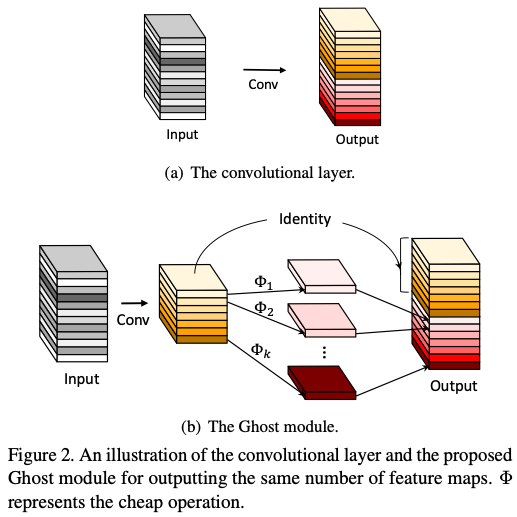
\includegraphics[scale=0.6]{src/img/Ghost module.jpg} \\
            \end{center}
            It is about to change the following equation for CNN layers: \\
            $$
                Y = X * f + b
            $$
            to, 
            $$
                Y^{\prime} = X * f^{\prime}
            $$
            where $f^{\prime} \in \mathcal{R}^{c \times k \times k \times m}$ is the utilized filters, and for $Y^{\prime}$ here goes,
            $$
                y_{ij} = \Phi_{i,j}(y_i^{\prime}), \forall i = 1,...,m, j = 1,...,s,
            $$
            where $ y_i^{\prime} $ is the i-th intrinsic feature map in $ Y^{\prime} $, $ \Phi_{i,j} $ in the
            above function is the j-th (except the last one) linear operation for generating the j-th ghost feature map $ y_{ij} $. \\

        \subsection{
            Applications
        }
            \subsubsection{
                Ghost Bottlenecks
            }   
                \begin{center}
                    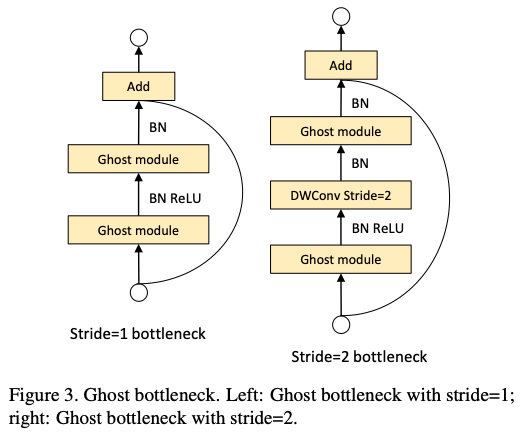
\includegraphics[scale=0.6]{src/img/Ghost bottleneck.jpg} \\
                \end{center}
                In practice, the primary convolution in Ghost module here is pointwise convolution for its efficiency. \\

            \subsubsection{
                GhostNet
            }
                Use the structure of \href{https://arxiv.org/pdf/1905.02244.pdf}{MobileNetV3} but re- place the bottleneck block in MobileNetV3 with our Ghost bottleneck. \\ 
                Also, there is a kind of GhostNet with width multiplier $ \alpha $ called GhostNet-$\alpha \times$. $\alpha$ here is a factor on the number of channels uniformly at each layer, To customize
                the network for smaller and faster models or higher accuracy on specific tasks. \\
                Width multiplier can control the model size and the computational cost quadratically by roughly $ \alpha^2 $. Usually smaller $\alpha$ leads to lower latency and lower performance, and vice versa. \\
        
    \section{
        Experiments
    }
        \subsection{
            setup
        }
            dataset: CIFAR-10, ImageNet ILSVRC 2012 dataset, MS COCO object detection benchmark. \\

        \subsection{
            Visualization of Feature Maps
        }
            \begin{center}
                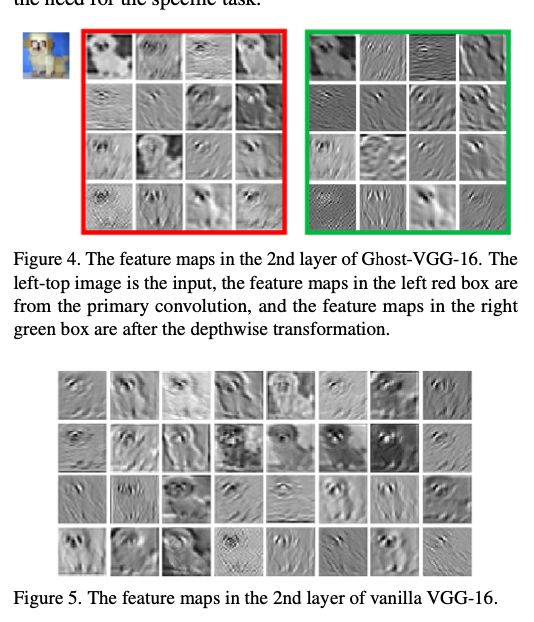
\includegraphics[scale=0.4]{src/img/FMaps.jpg} \\
            \end{center}
        
        \subsection{
            Comparison
        }
            \subsubsection{
                CIFAR-10
            }
                \begin{center}
                    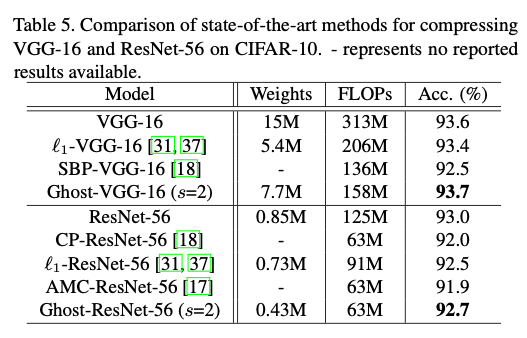
\includegraphics[scale=0.4]{src/img/Com_cifar10.jpg} \\
                \end{center}
            \subsubsection{
                ImageNet
            }
                \begin{center}
                    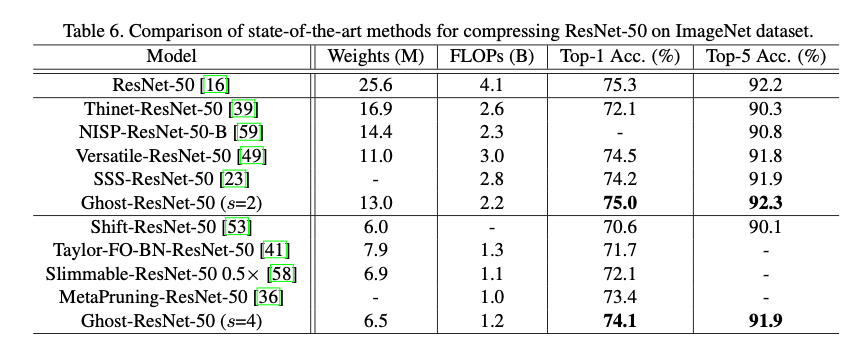
\includegraphics[scale=0.4]{src/img/Com_imagenet.jpg} \\
                \end{center}
            \subsubsection{
                Visual Benchmarks
            }
                \begin{center}
                    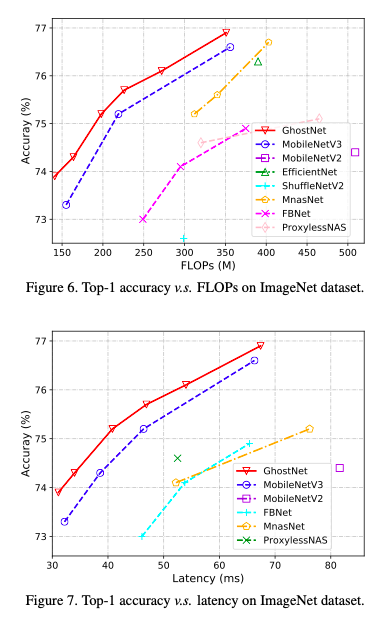
\includegraphics[scale=0.4]{src/img/acc_and_lat.jpg} \\
                    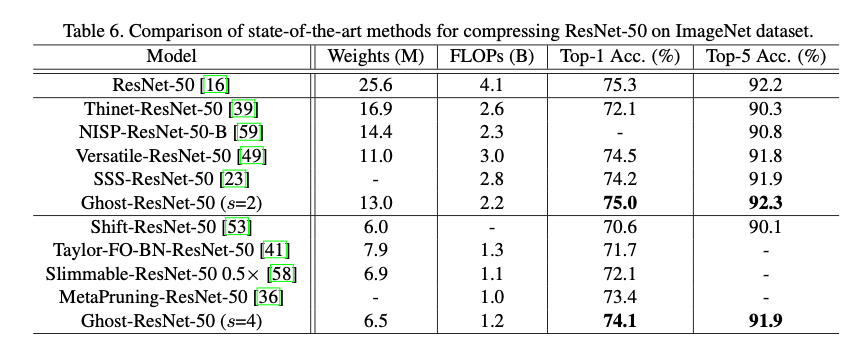
\includegraphics[scale=0.4]{src/img/Com_imagenet.jpg} \\
                \end{center}
            \subsubsection{
                MS COCO
            }
                \begin{center}
                    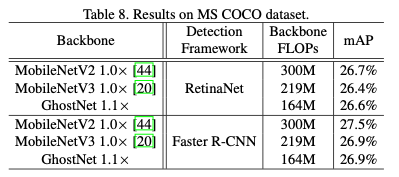
\includegraphics[scale=0.6]{src/img/MSCOCO.jpg} \\
                \end{center}                

\end{document}